\documentclass[11pt,aspectratio=43]{beamer}
\usepackage[utf8]{inputenc}
\usepackage{amsmath, amsfonts, amssymb, amsthm}
\usepackage[T1]{fontenc}
\usepackage{lmodern}
\usepackage{xcolor}
\usepackage{setspace}
\usepackage{booktabs}
\usepackage{multirow}
\usepackage{graphicx}
\usepackage{pgfplots}
\usepackage{tikz}
\usetikzlibrary{intersections}
\usetikzlibrary{decorations}
\usetikzlibrary{decorations.pathreplacing}
\usepackage{ulem}
\usepackage{hyperref}
\usepackage{booktabs}
\usepackage{babel}
\usepackage{makecell}
\usepackage[para,online,flushleft]{threeparttable}
\usepackage{pdfpages}
\usepackage{tcolorbox}
\usepackage{bm}
\usepackage{appendixnumberbeamer}
\usepackage{natbib}
\usepackage{caption}
\captionsetup[figure]{labelformat=empty}% redefines the caption setup of the figures environment in the beamer class.
\usetheme[compress]{Boadilla}
\usecolortheme{default}
\useoutertheme{miniframes}
\usefonttheme[onlymath]{serif}

\newcommand{\jump}[2]{\hyperlink{#1}{\beamerbutton{#2}}}
\newcommand{\orange}[1]{\textcolor{orange}{#1}}
\newcommand{\red}[1]{\textcolor{red}{#1}}

\setbeamertemplate{itemize item}{\raisebox{0.1em}{\scalebox{0.7}{$\blacksquare$}}}
\setbeamertemplate{itemize subitem}[circle]
\setbeamertemplate{itemize subsubitem}{--}
\setbeamercolor{itemize item}{fg=black}
\setbeamercolor{itemize subitem}{fg=black}
\setbeamercolor{itemize subsubitem}{fg=black}
\setbeamercolor{item projected}{bg=darkgray,fg=white}
\definecolor{blue}{rgb}{0.2, 0.2, 0.7}
\setbeamercolor{alerted text}{fg=blue}
\setbeamertemplate{enumerate items}[circle]


\setbeamertemplate{headline}{}

%==========================================
\let\olditemize=\itemize
\let\endolditemize=\enditemize
\renewenvironment{itemize}{\olditemize \itemsep1em}{\endolditemize}
\let\oldenumerate=\enumerate
\let\endoldenumerate=\endenumerate
\renewenvironment{enumerate}{\oldenumerate \itemsep1em}{ \endoldenumerate}

\DeclareMathOperator*{\argmax}{\arg\!\max}
\DeclareMathOperator*{\E}{\mathbb{E}}
\DeclareMathOperator*{\var}{\rm Var}
\DeclareMathOperator*{\cov}{\rm Cov}

\theoremstyle{definition}
\newtheorem{assume}{Assumption}
\newtheorem{lem}{Lemma}
\newtheorem{proposition}{Proposition}
\newtheorem{thm}{Theorem}
\newtheorem{corol}{Corollary}

\begin{document}
    \title[Lecture 4]{Lecture 4 \\ Representative Consumer \\ Preference and Constraints }
    \author[Hui-Jun Chen]{Hui-Jun Chen}
    \institute[OSU]{The Ohio State University}
    % \date{\today}
    \date{\today}
    \setbeamertemplate{navigation symbols}{}
    \setstretch{1.2}

%-------------------------------------------------------
{
%	\usebackgroundtemplate{\includegraphics[width=1\paperwidth]{../EveningSky_cropped_edit43_bright.jpg}}
    \begin{frame}
% \vspace{3em}
        \centering
%		{\footnotesize 	ECON 4002 Intermediate Macroeconomic Theory}
        \maketitle
% \vspace{-1.5em}
% \centering
% \includegraphics[width=0.55\linewidth]{Pictures/houses.jpeg}


    \end{frame}
}

% -------------------------------------------
\setbeamertemplate{headline}
{
\setbeamercolor{section in head/foot}{fg=black, bg=white}
\vskip1em \tiny \insertsectionnavigationhorizontal{1\paperwidth}{\hspace{0.50\paperwidth}}{}
}
%------------------------------------------

\begin{frame}{Overview: Lecture 4 - 7}
\label{slide:Overview__Lecture_4_7}

\begin{center}
Provide \alert{micro-foundation} for the \alert{macro implication} (\alert{Lucas critique})
\end{center}

\begin{itemize}
    \item \textbf{Representative Consumer}:
    \begin{itemize}
        \item Lecture 4: \alert{preference}, \alert{constraints}
        \item Lecture 5: \alert{optimization}, \alert{application}
        \item Lecture 6: Numerical Examples
    \end{itemize}
    \item \textbf{Representative Firm}:
    \begin{itemize}
        \item Lecture 7: \alert{production}, \alert{optimization}, \alert{application}
    \end{itemize}
\end{itemize}
\end{frame}

\section{Preference}
\label{sec:Preference}

\begin{frame}{Utility Function}
\label{slide:Utility_Function}
    We use utility function $ U( C, l ) $ to represent the \alert{preference/happiness}
    \begin{itemize}
        \item $ C $: consumption (assume single/composite goods)
        \item $ l $: leisure (time spent not working)
    \end{itemize}
    Utility function defines the \alert{ranking} of \alert{$(C, l)$ bundles}
    \begin{itemize}
        \item If $ U( C_{1}, l_{1} ) > U( C_{2}, l_{2} ) $, then $ ( C_{1}, l_{1} ) $ is \alert{strictly preferred} to $ ( C_{2}, l_{2} ) $
        \begin{itemize}
            \item $ \because $ $( C_{1}, l_{1} ) $ bundle generate \alert{more} happiness than $ ( C_{2}, l_{2} ) $ bundle
        \end{itemize}
        \item If $ U( C_{1}, l_{1} ) = U( C_{2}, l_{2} ) $, then \alert{indifferent} between $ ( C_{1}, l_{1} ) $ and $ ( C_{2}, l_{2} ) $
        \begin{itemize}
            \item $ \because $ $( C_{1}, l_{1} ) $ bundle generate \alert{same} happiness as $ ( C_{2}, l_{2} ) $ bundle
        \end{itemize}
        \item Note: \alert{level} of utility is meaningless, only \alert{order} matters!
    \end{itemize}
\end{frame}

\begin{frame}{Properties of Utility Function}
\label{slide:Properties_of_Utility_Function}
    \begin{enumerate}
        \item \textbf{Monotonicity}: more is always better!
        \begin{itemize}
            \item If $ C_{1} > C_{2} $ and $ l_{1} > l_{2} $, then $ U( C_{1}, l_{1} ) > U( C_{2}, l_{2} ) $
        \end{itemize}
        \item \textbf{Convexity}: prefer \alert{diversified} consumption bundles
        \begin{itemize}
            \item e.g. prefer food $ + $ leisure rather than overeating / oversleeping
        \end{itemize}
        \item \textbf{Normality}: consumption and leisure are \alert{normal} goods
        \begin{itemize}
            \item income $ \uparrow  $ $ \Rightarrow  $ consumption $ \uparrow  $
            \item leisure is complicated: relates to income
            \begin{itemize}
                \item the poor: less leisure means \alert{more} labor income
                \item the rich: more income means \alert{more} leisure
            \end{itemize}
        \end{itemize}
    \end{enumerate}
\end{frame}

\begin{frame}{Rep. of Utility Function: Indifference Curve}
\label{slide:Representation_of_Utility_Function__Indifference_Curve}
\begin{columns}
    \begin{column}{0.5\textwidth}
        \begin{itemize}
            \item \textbf{Def}: $ ( C, l ) $ bundles that yield \alert{the same} utility level
            \item \alert{Monotonicity} $ \Rightarrow  $ downward sloping
            \item \alert{Convexity} $ \Rightarrow  $ diversity shown in comparison between point $ B $ and $ D $
        \end{itemize}
    \end{column}
    \begin{column}{0.5\textwidth}
        \begin{figure}
            \caption{Figure 4.1 Indifference Curves}
            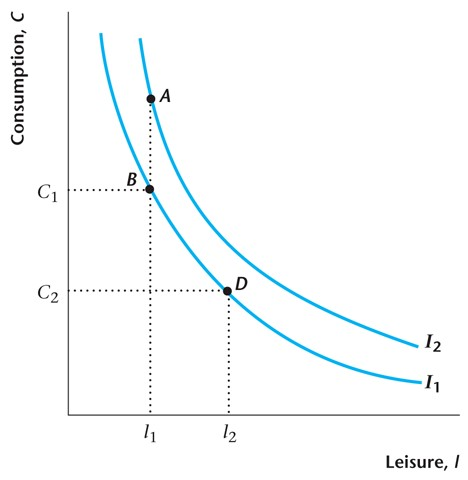
\includegraphics[width=\textwidth]{./figures/Figure4_1.jpg}
        \end{figure}
    \end{column}
\end{columns}
\end{frame}

\begin{frame}{Rep. of Utility Function: Indifference Curve (Cont.)}
\label{slide:Rep_of_Utility_Function__Indifference_Curve__Cont__}
\framesubtitle{\jump{slide:Note_on_Calculus}{Calculus}}
    \begin{columns}
        \begin{column}{0.5\textwidth}
            \begin{itemize}
                \item \alert{Normality}: M{\tiny arginal}R{\tiny ate of }S{\tiny ubstitution}
                \begin{itemize}
                    \item \textbf{Marginal}: for \alert{arbitrary small} change in $ x $-axis (leisure in this case)
                    \item \textbf{rate of substitution}: the amount on $ y $-axis has to be sacrificed (consumption in this case)
                \end{itemize}
                %
                \begin{equation}
                \label{eq:MRS}
                    MRS_{l, C} = \frac{D_{l} U( C, l )}{D_{C}U( C, l )}
                ,\end{equation}
                %
                where $ D_{x}U( \cdot ) $ is derivative of $ U $ w.r.t. $ x $
            \end{itemize}
        \end{column}
        \begin{column}{0.5\textwidth}
        \begin{figure}
            \caption{Figure 4.2 MRS}
            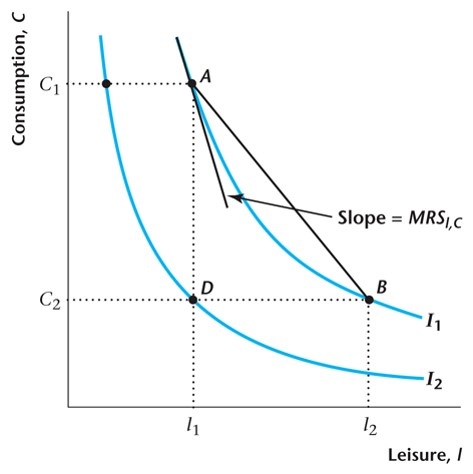
\includegraphics[width=\textwidth]{./figures/Figure4_2.jpg}
        \end{figure}
        \end{column}
    \end{columns}
\end{frame}

\begin{frame}{Computing MRS}
\label{slide:Computing_MRS}
    \begin{columns}
        \begin{column}{0.6\textwidth}
            \begin{itemize}
                \item little change in leisure $ dl > 0 $ $ \Rightarrow  $ change in utility $ D_{l}U( C, l ) dl $
                \item with the cost of income loss $ \Rightarrow  $ consumption has to drop by $ dC < 0 $ amount $ \Rightarrow  $ change in utility $ D_{C}U( C, l ) dC $
                \item Stay on the IC $ \Rightarrow  $ utility remain the same:
                %
                %
                \begin{align*}
                    D_{C} & U( C, l ) dC + D_{l}U( C, l ) dl = 0 \\
                   \frac{dC}{dl} & = - \frac{D_{l}U( C, l )}{D_{C} U( C, l )} = - MRS_{l, C}
                \end{align*}
                %
            \end{itemize}
        \end{column}
        \begin{column}{0.5\textwidth}
            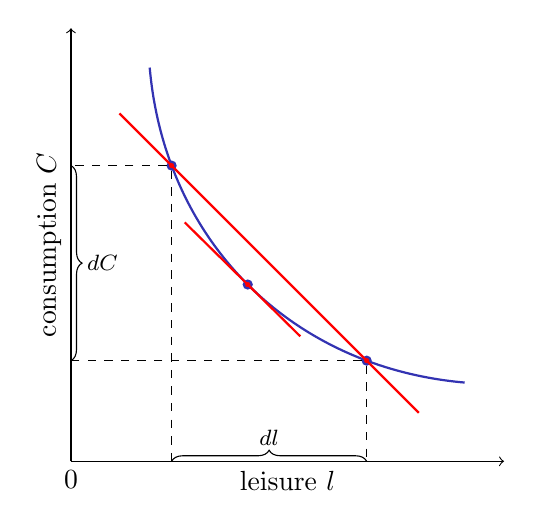
\begin{tikzpicture}
                \pgfmathsetmacro{\x}{5};
                \pgfmathsetmacro{\y}{5};
                % \draw[very thin,color=gray, step=0.1] (0,0) grid (\x, \y); % gray grid
                \draw[->] (0,0) node[below]{ $ 0 $  } -- node[below]{leisure $l$} (\x + 0.5,0) ;   % label x axis
                \draw[->] (0,0) -- node[above, rotate=90]{consumption $C$} (0,\y + 0.5) ;   % label y axis
                \draw[thick, blue] (1, \y) to[bend right=40]
                        node[pos=0.2,draw,fill=red,circle,inner sep=1pt] (a) {}
                        node[pos=0.8,draw,fill=red,circle,inner sep=1pt] (b) {}
                        node[pos=0.5,draw,fill=red,circle,inner sep=1pt] (c) {}
                        node[pos=0.51] (d) {}
                        (\x,1);

                \path (a); \pgfgetlastxy{\xaxis}{\yaxis};
                \coordinate (a_x) at (\xaxis, 0);
                \coordinate (a_y) at (0, \yaxis);
                \draw[dashed] (a) -- (a_x);
                \draw[dashed] (a) -- (a_y);

                \path (b); \pgfgetlastxy{\xaxis}{\yaxis};
                \coordinate (b_x) at (\xaxis, 0);
                \coordinate (b_y) at (0, \yaxis);
                \draw[dashed] (b) -- (b_x);
                \draw[dashed] (b) -- (b_y);


                \draw [decorate,decoration={brace,amplitude=4pt},xshift=0pt,yshift=3pt]
                       (a_x) -- (b_x) node [black,midway,yshift=.3cm] {\footnotesize $dl$};
                \draw [decorate,decoration={brace,amplitude=4pt},xshift=3pt,yshift=0pt]
                       (a_y) -- (b_y) node [black,midway,xshift=.4cm] {\footnotesize $dC$};
                \draw[shorten >=-1cm, shorten <=-1cm, thick, red] (a) -- (b);
                \draw[shorten >=-1cm, shorten <=-1cm, thick, red] (c) -- (d);
            \end{tikzpicture}
        \end{column}
    \end{columns}
\end{frame}

\begin{frame}{Algebraic Example}
\label{slide:Algebraic_Example}
    Suppose $ U( C, l ) = \frac{C^{1-\sigma}}{1-\sigma} + \psi \ln l $, where $ \sigma $ and $ \psi $ are parameters. Then,
    \begin{itemize}
        \item $D_{C} U( C, l ) = ( 1-\sigma) \frac{C^{1-\sigma - 1}}{1-\sigma} = C^{-\sigma}$
        \item Remember $ \frac{d \ln l}{dl} = \frac{1}{l} $, $ D_{l} U( C, l ) = \frac{\psi}{l}$
        \item $ MRS_{l, C} = \frac{D_{l} U( C, l )}{D_{C}U( C, l )} = \frac{\psi}{l C^{-\sigma}} $
    \end{itemize}
\end{frame}

\section{Constraints}
\label{sec:Constraints}

\begin{frame}{Budget Constraints}
\label{slide:Budget_Constraints}
    \begin{itemize}
        \item \textbf{Time}: consumer has $ h $ hours per day, and allocate between leisure $ l $ and labor supply $ N^{s} $
        %
        \begin{equation}
        \label{eq:LaborTime}
            l + N^{s} = h
        \end{equation}
        %
        \item \textbf{Budget}: consumer cannot spend more than the income he/she has
        \begin{itemize}
            \item \alert{labor income}: wage rate $ w $ times labor supply $ N^{s} $, $ wN^{s} $
            \item \alert{dividends income}: consumer buys share of the firm, gain dividend $ \pi $
            \item \alert{tax}: consumer is subject to lump-sum taxes $ T $
        \end{itemize}
        %
        \begin{equation}
        \label{eq:budgetConstraint}
            C \le w N^{s} + \pi - T
        \end{equation}
        %
        \item Consumption is \textbf{numeraire}: price \alert{normalized} to $ 1 $.
        \begin{itemize}
            \item Imagine consumption goods as \alert{unit of account}, ppl directly trade with consumption goods
        \end{itemize}
    \end{itemize}
\end{frame}

\begin{frame}{Visualization of Budget Set}
\label{slide:Visualization_of_Budget_Set}
    \begin{columns}
        \begin{column}{0.5\textwidth}
            \begin{figure}
                \caption{Figure 4.3 Representative Consumer's Budget Constraint when $ T > \pi $ (``poor'')}
                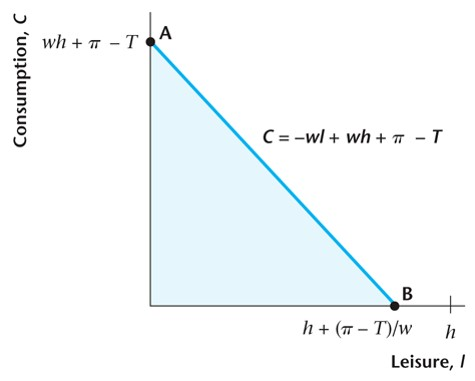
\includegraphics[width=\textwidth]{./figures/Figure4_3.jpg}
            \end{figure}
        \end{column}
        \begin{column}{0.5\textwidth}
            \begin{figure}
                \caption{Figure 4.4 Representative Consumer's Budget Constraint when $ T < \pi $ (``rich'')}
                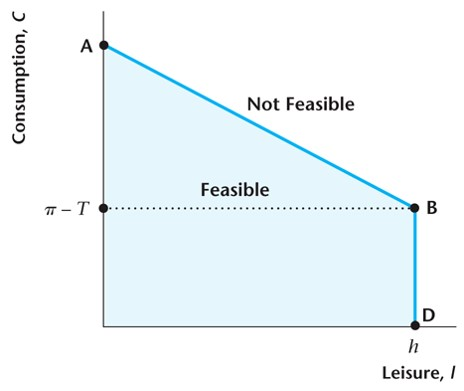
\includegraphics[width=\textwidth]{./figures/Figure4_4.jpg}
            \end{figure}
        \end{column}
    \end{columns}
\end{frame}

\section{Appendix}
\label{sec:Appendix}

\appendix
% -------------------------------------------
\setbeamertemplate{headline}
{
\setbeamercolor{section in head/foot}{fg=black, bg=white}
\vskip1em \tiny \insertsectionnavigationhorizontal{1\paperwidth}{\hspace{0.50\paperwidth}}{}
}
%------------------------------------------
\begin{frame}\frametitle{}
\begin{columns}
\label{Appendix}
\column{1\linewidth}
\centering
{\Large \alert{Appendix}}
\end{columns}
\end{frame}

\section{Calculus}
\label{sec:Calculus}



\begin{frame}{Note on Calculus}
\label{slide:Note_on_Calculus}
\framesubtitle{\jump{slide:Rep_of_Utility_Function__Indifference_Curve__Cont__}{Back}}
    \begin{itemize}
	\item Function: $y = f\left( x \right) $, how $ y $ is determined by $ x $
	    \begin{itemize}
	        \item E.g.,  $y = 3x+2$: if $x=3$, then $3$ times  $3$ and plus $2$ will get $y=11$
	    \end{itemize}
	\item Differentiation: how changes in $ x $ results in change in $y$
	    \begin{itemize}
	        \item E.g., $y = 3x+2$,
		    \begin{table}[htpb]
		        \centering
		        \caption{Table for how the value of $x$ affects the value of $y$}
		        \label{tab:Table-for-how-the-value-of-x-affects-the-value-of-y-}
		        \begin{tabular}{cccccc}
			    $x$ & $1$ &  $2$ &  $3$ & $4$ & $5$ \\
			    \hline
			    $y$ & $5$ & $8$ & $11$ & $14$ & $17$ \\
		        \end{tabular}
		    \end{table}
		    \textbf{Notice $ \Delta x = 1 \implies  \Delta y = 3  \implies  \frac{ \Delta y}{ \Delta x} = 3 $}, change to differentiation notation, $\frac{dy}{dx}  = 3$
	    \end{itemize}
	\item  \textbf{Tips}: $y = 3x^{2} + 9x  + 2 $, look at terms with $x$,  $dy = 3 \times 2 x\left( dx \right) + 9 \left( dx \right)   \implies \frac{dy}{dx} = 6x+9  $
    \end{itemize}
\end{frame}



\end{document}

